\section{Simulation et tests}

Cette partie contient les différents tests et simulations effectuées au cours du projet

\subsection{Contrôle des timings}
J'ai utilisé vsim afin de contrôler que mes timings étaient bons en me basant sur les timings montrés dans le document "Designing a AXI4-lite Slave Peripheral, Griffin, Xilinx", qui sont les suivants : 

\begin{figure}[ht]
	\centering
	\begin{minipage}{.5\textwidth}
		\centering
		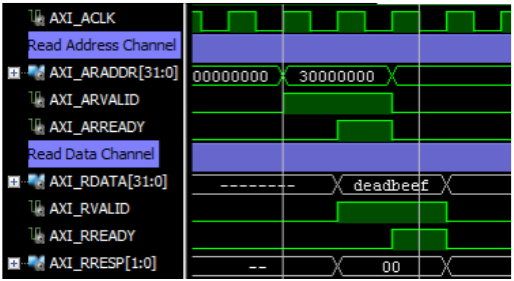
\includegraphics[scale=0.4]{./images/timing_read.png}
		\captionof{figure}{Laboratoire 5 : Timing read}
	\end{minipage}%
	\begin{minipage}{.5\textwidth}
		\centering
		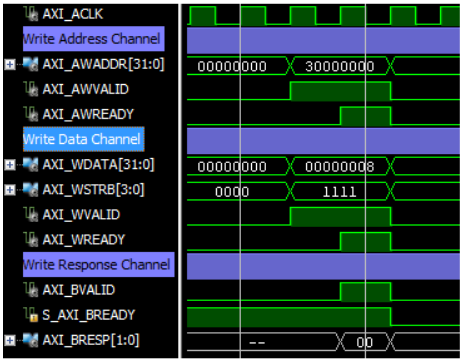
\includegraphics[scale=0.4]{./images/write_timing.png}
		\captionof{figure}{Laboratoire 5 : Timing write}
	\end{minipage}
\end{figure}

Et maintenant, voici les timings que j'ai obtenus lors de la simulation : \\

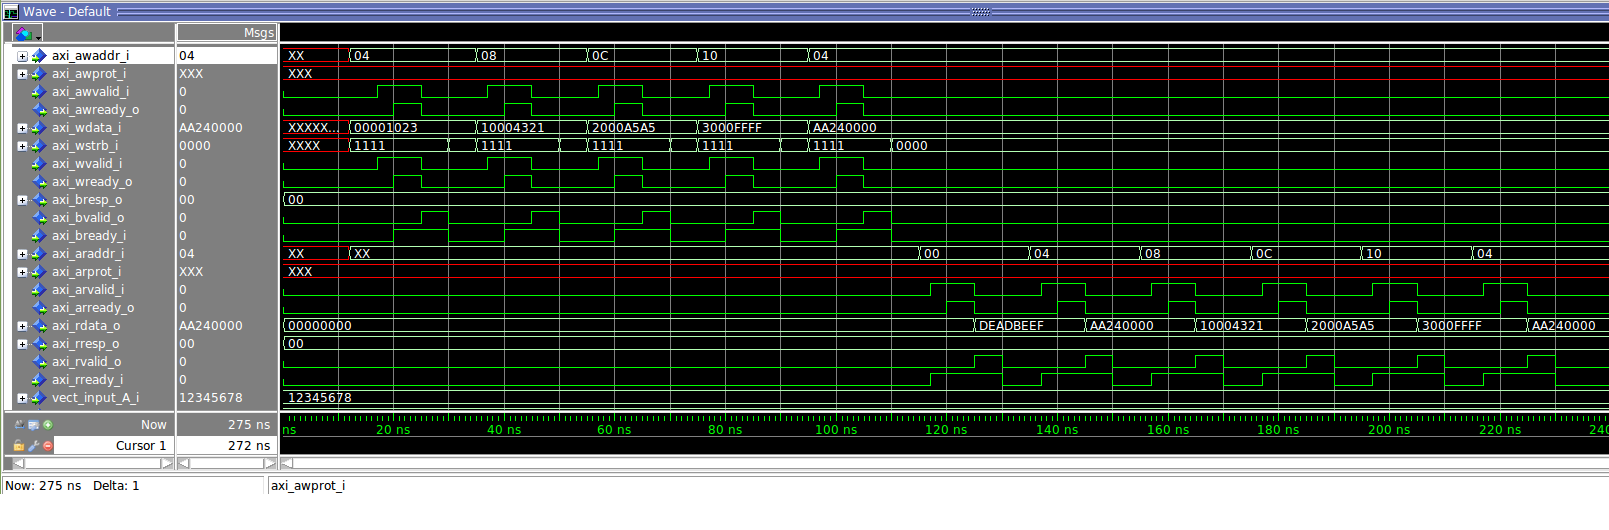
\includegraphics[scale=0.3]{./images/vsim_base_timing.png}
\captionof{figure}{Laboratoire 5 : Timing implémentation bus axi lite}

On peut voir que le timing du read correspond au timing voulu à l'exception du fait que dans notre cas la durée d'activation d'axi\_rvalid et de axi\_bready est inversé. Cela n'impacte pas le fonctionnement du programme, les deux signaux se retrouvant désactivés au même moment.Par contre, le timing du canal de réponse du write est décalé d'un coup d'horloge. Cela n'a pas d'impact sur le fonctionnement du bus, étant donnée que dans le cadre l'écriture, nous pouvons nous permettre de prendre un peu plus de temps, car on nous fournit une donnée que nous devons stocker, ce n'est pas nous qui devons fournir la donnée sur le bus de lecture. \\\\
L'écriture et la lecture fonctionnent correctement dans cette simulation, les registres et bus étant mis à jour et les timings respectés.
\subsection{Test du strobe}
En modifiant le testbench, il était possible de réaliser des tests sur le fonctionnement du strobe. Voici les résultats obtenus : \\

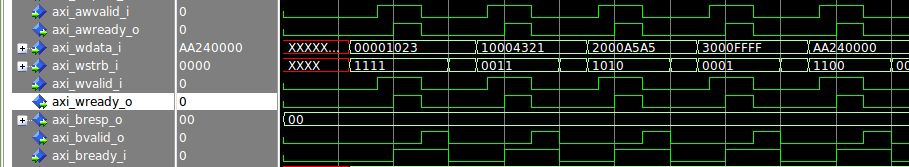
\includegraphics[scale=0.5]{./images/write_strb.png}
\captionof{figure}{Laboratoire 5 : Write avec différents strobes}

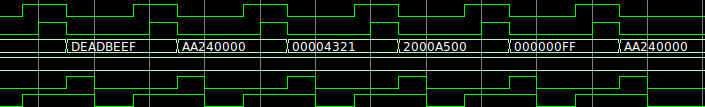
\includegraphics[scale=0.6]{./images/read_strobe.png}
\captionof{figure}{Laboratoire 5 : Read après different strobes}

Je rends attentif ici au fait que le registre à l'offset 04 est écrit deux fois, une fois au tout début de la phase d'écriture et une fois à la fin de la phase d'écriture, ce qui explique la valeur 0xAA240000 lue, valeur qui respecte le strobe qui lui était attribué (1100). On peut voir que les valeurs respectent les strobes qui ont été utilisés lors de l'écriture quand on les lit.

\subsection{Problèmes rencontrés}

Durant ce laboratoire, j'ai rencontré un problème principal, qui était un problème de timing. Pour imager cela, je vais insérer ici une image présentant la phase de debug que j'ai dû effectuer pour m'en rendre compte. J'ai utilisé SignalTap 2 : \\
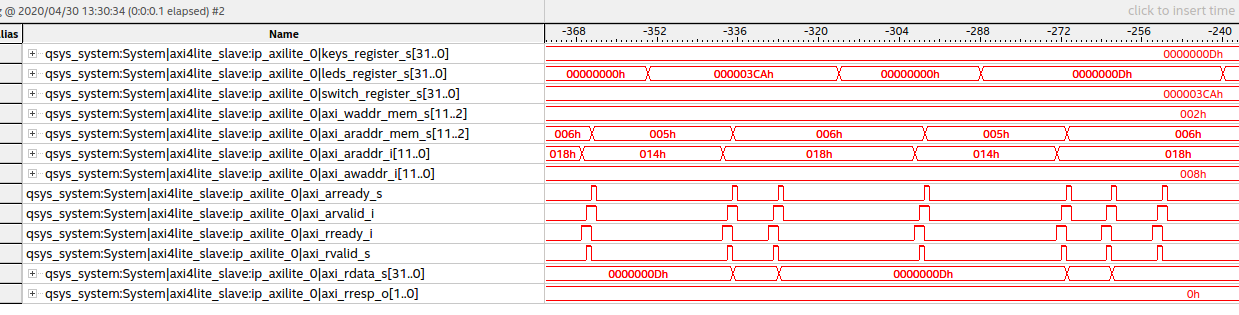
\includegraphics[scale=0.38]{./images/signaltap.png}
\captionof{figure}{Laboratoire 5 : Read Signal Tap 2}

On peut voir que les signaux arready et arrvalid sont activés après les signaux rready et rvalid, ce qui au vu des timings étudiés plus tôt représente une erreur d'implémentation. J'ai pu régler ce problème dans le code VHDL par la suite, pour arriver à l'implémentation finale qui vous a été présentée.

\subsection{Tests sur board}

Voici les tests effectués sur la board : \\

Comme dans le dernier laboratoire, j'ai commencer par effectuer un appui sur key 0 et un appui sur key 1 en gardant les switchs down : \\\\
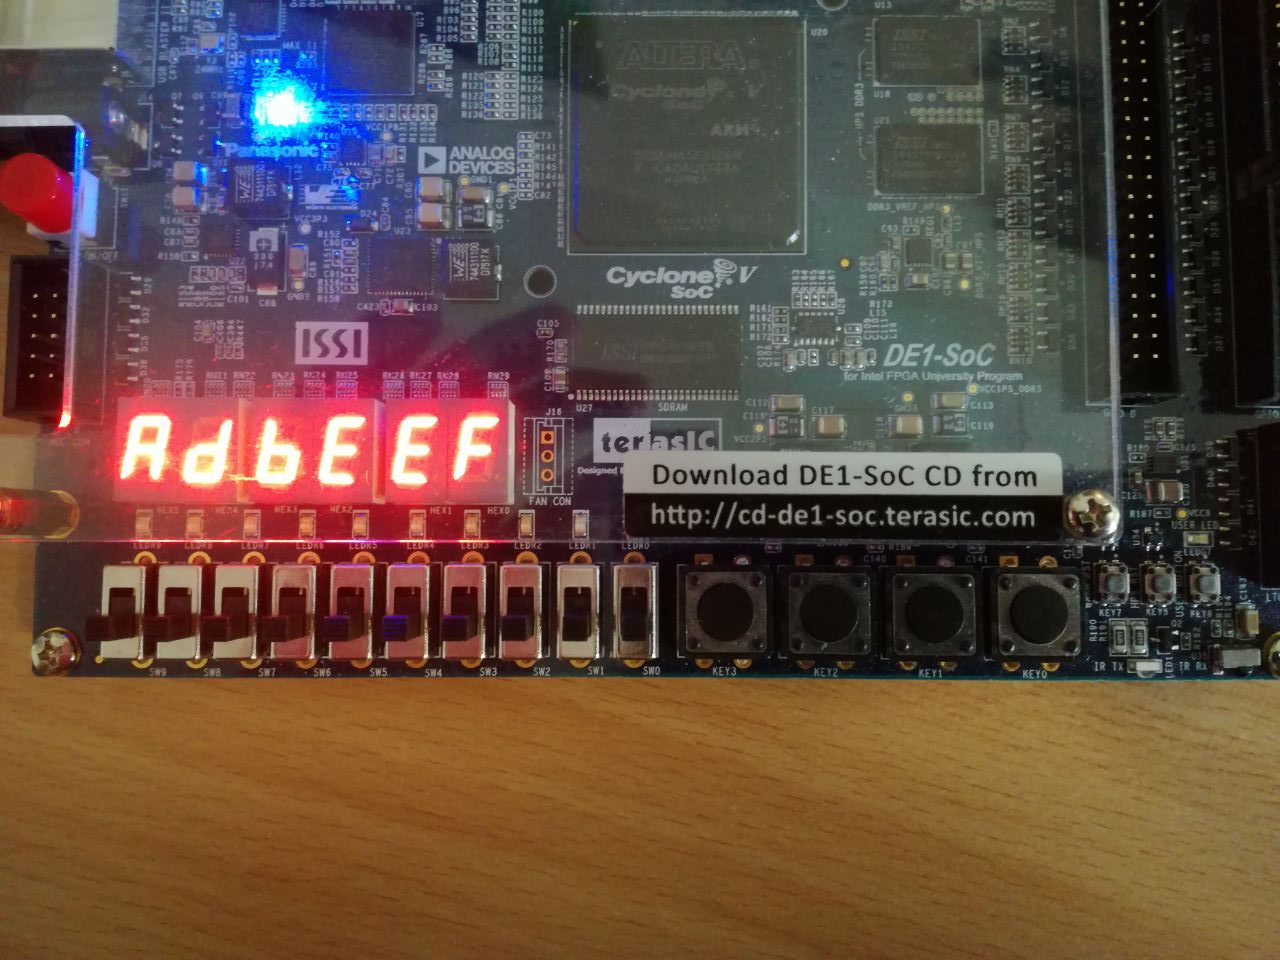
\includegraphics[scale=0.3]{./images/testp1.jpeg}
\captionof{figure}{Laboratoire 5 : Appuis sur key 0, switch down}

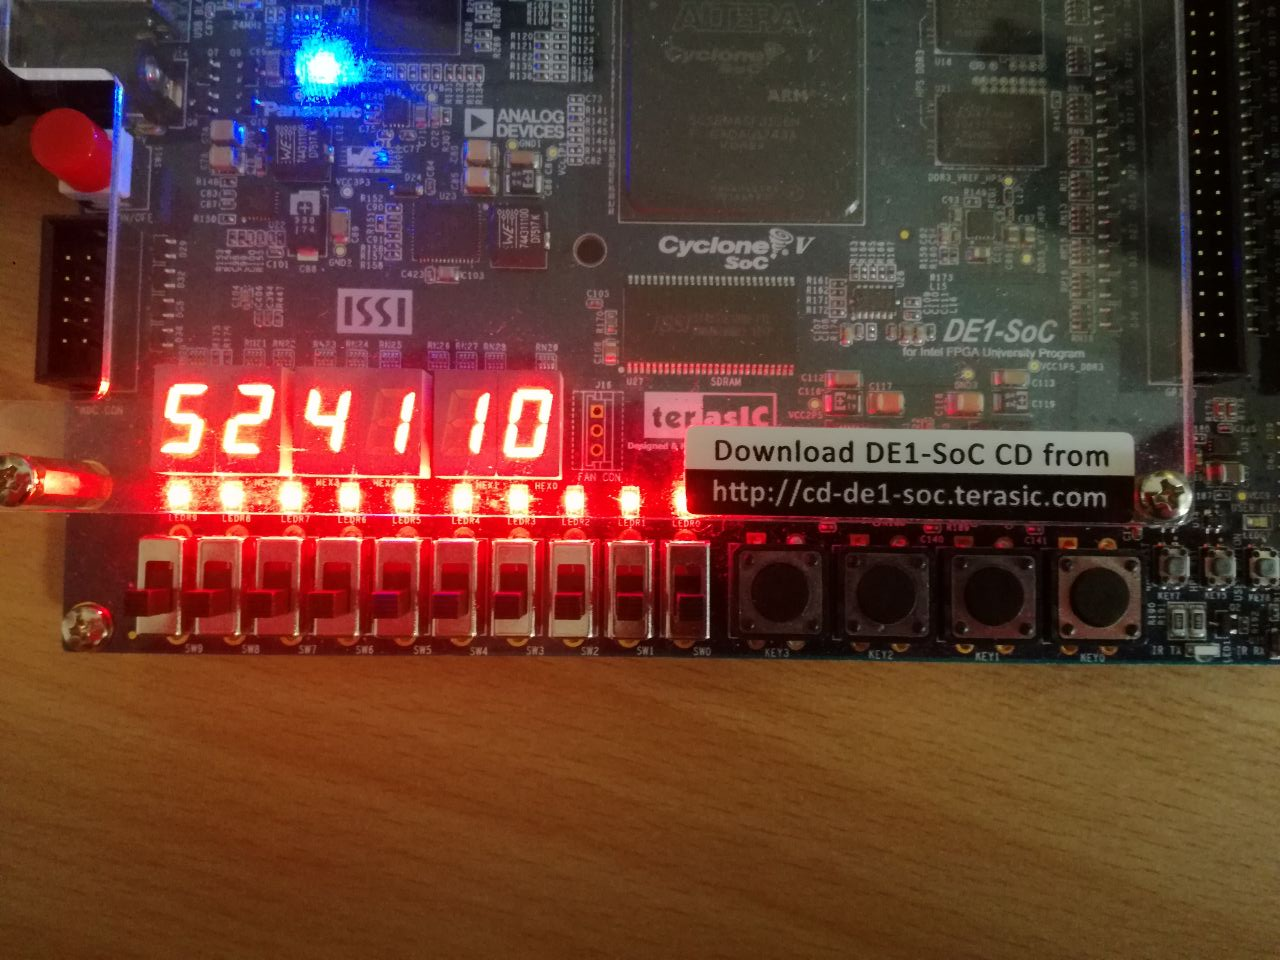
\includegraphics[scale=0.3]{./images/testp2.jpeg}
\captionof{figure}{Laboratoire 5 : Appuis sur key 1, switch down}

La spécification des leds est respectée, ainsi que la spécification des afficheurs 7 segments. la constante étant (0xDEADBEEF), on voit apparaître l'état des bits 23 à 0 dans le cas d'un appui sur key 0 (ADBEEF), et l'état inverse dans le cas d'un appui sur key 1.J'ai par la suite alterné les switch en en laissant un up et un down, en commencant avec le switch 9 down, et j'ai répéter la même action qu'auparavant :

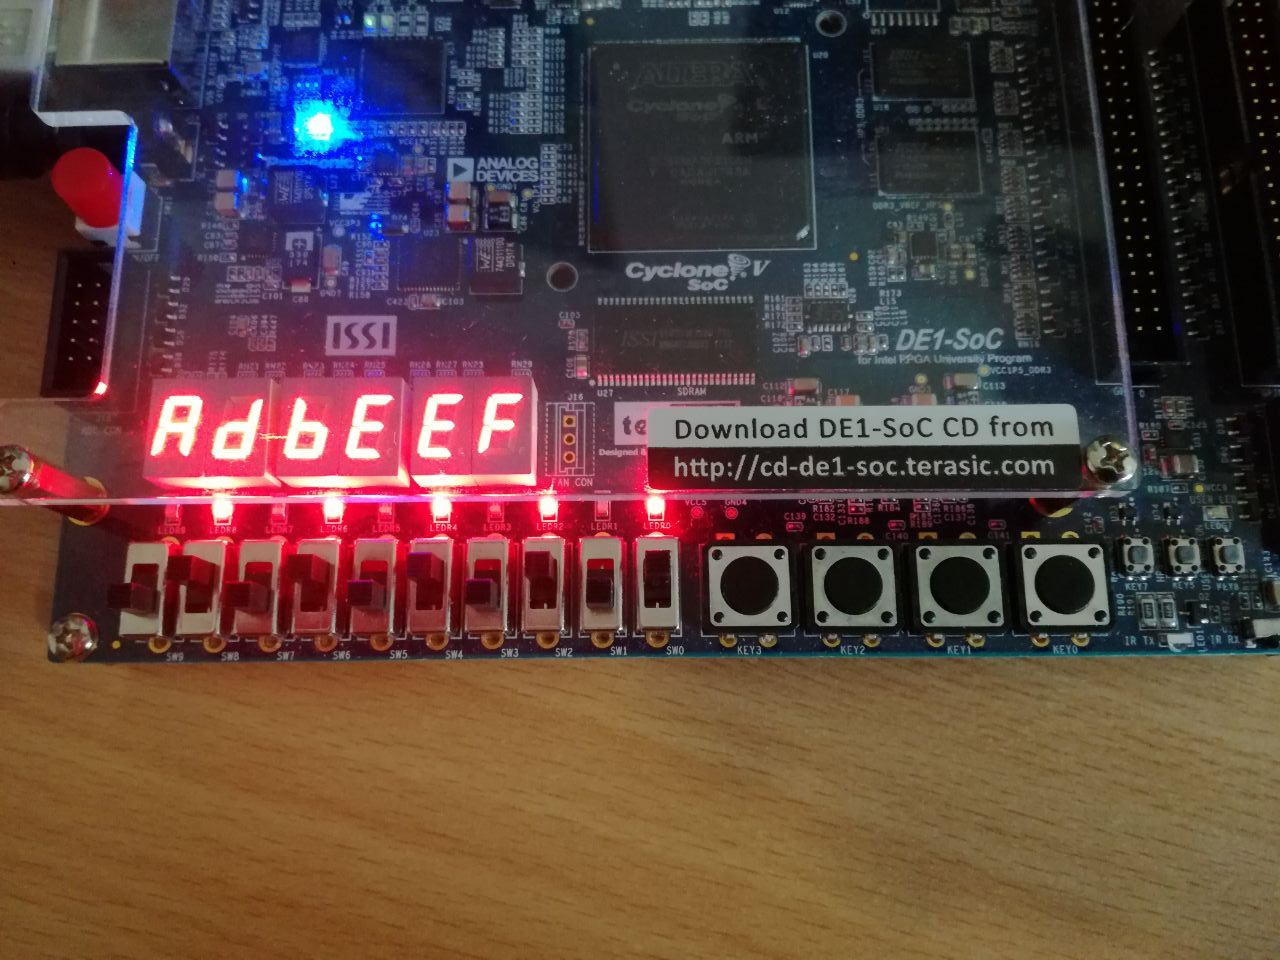
\includegraphics[scale=0.3]{./images/testp3.jpeg}
\captionof{figure}{Laboratoire 5 : Appuis sur key 0, switch alternés}

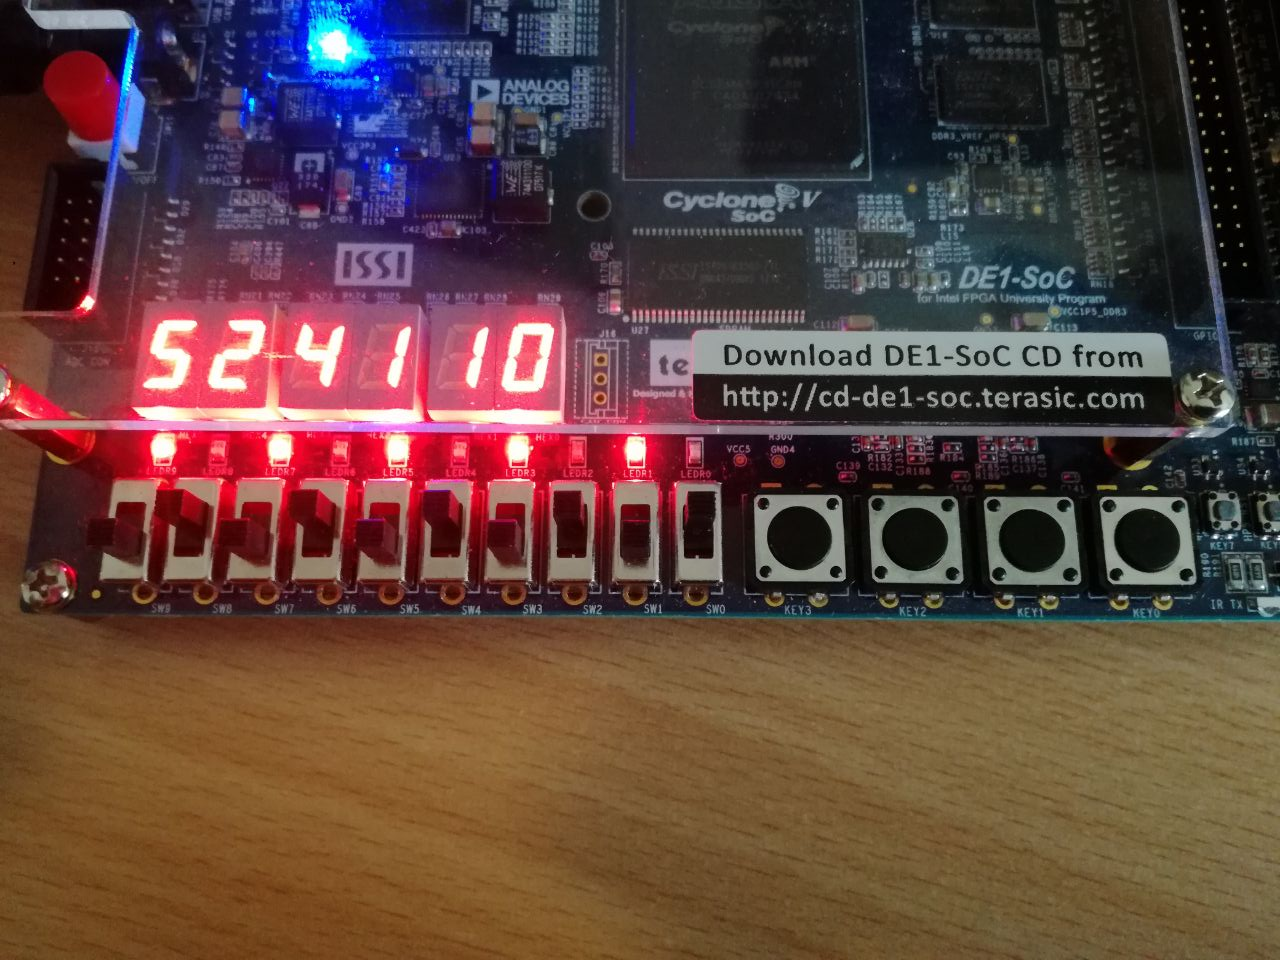
\includegraphics[scale=0.3]{./images/testp4.jpeg}
\captionof{figure}{Laboratoire 5 : Appuis sur key 1, switch alternés}
On peut voir ici que le fonctionnement est correct. J'ai finalement testé les interruptions en appuyant 2 fois sur le bouton key 3 puis 1 fois sur le bouton key 2 : \\

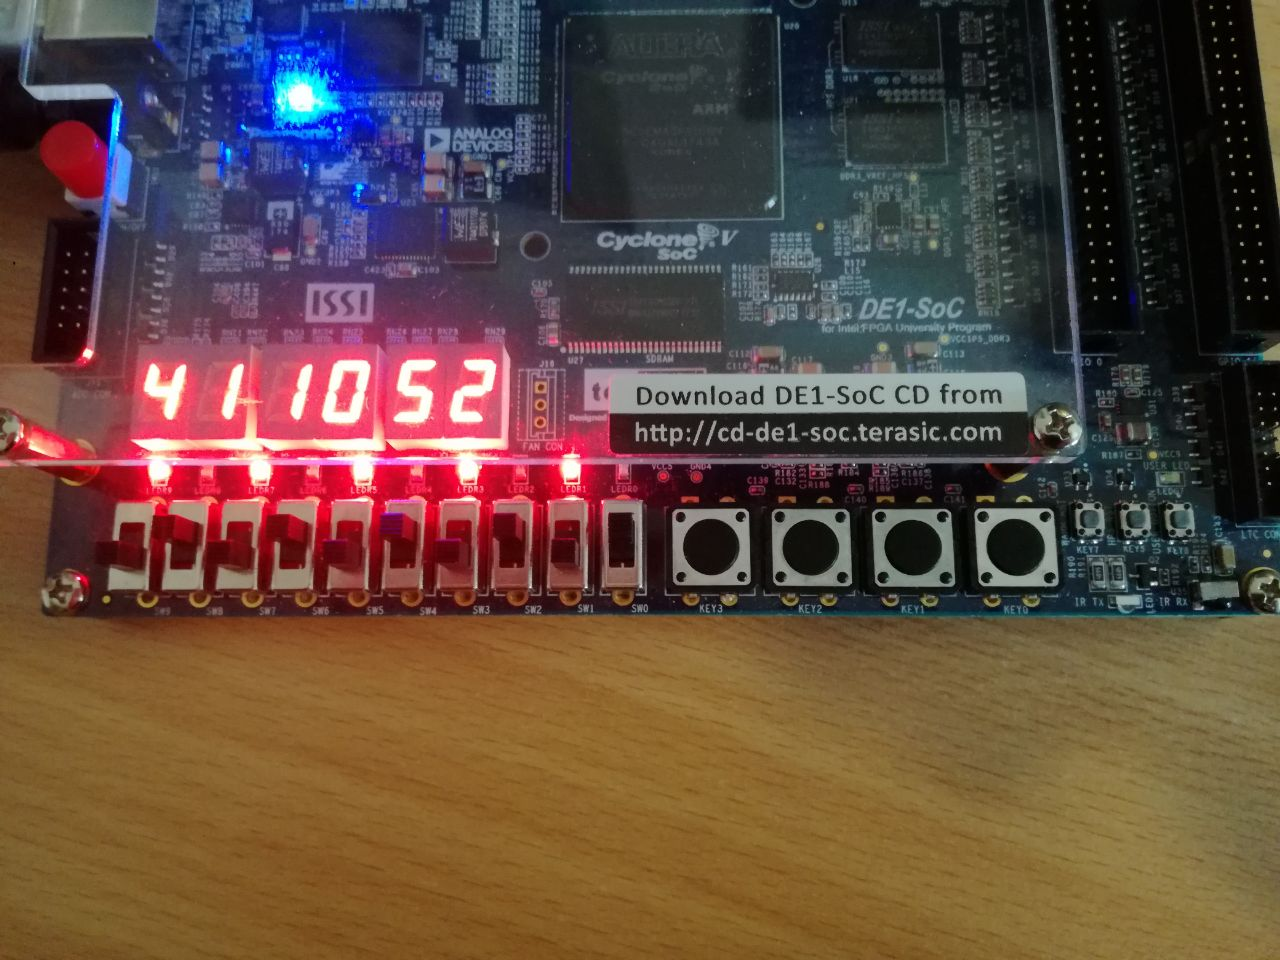
\includegraphics[scale=0.3]{./images/testp5.jpeg}
\captionof{figure}{Laboratoire 5 : 2 Appuis sur key 3}

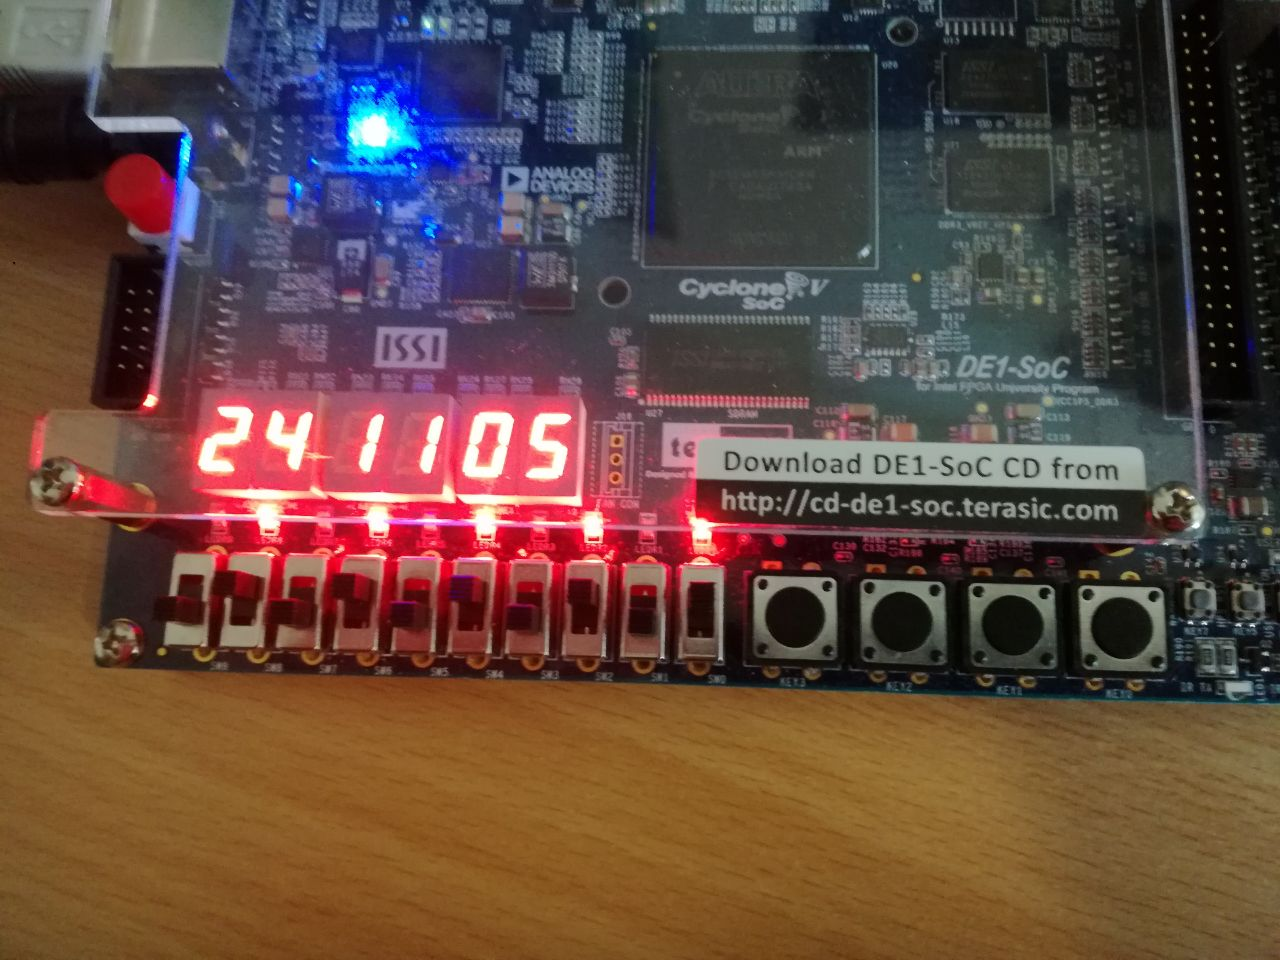
\includegraphics[scale=0.3]{./images/testp6.jpeg}
\captionof{figure}{Laboratoire 5 : 1 Appuis sur key 2}

Ici à nouveau, le fonctionnement est correct et le résultat correspond à la spécification fournie.